\documentclass[a4paper,14pt,russian]{extreport}

%Чтобы работали все шрифты
\usepackage{extsizes}
%\usepackage{cmap} % для кодировки шрифтов в pdf
\usepackage[T2A]{fontenc}
\usepackage[utf8]{inputenc}
\usepackage[russian]{babel}

%Таблицы
\usepackage{booktabs}

%Для рисуночков
%\usepackage[pdftex]{graphicx}
%\graphicspath{{figures/}}
%\DeclareGraphicsExtensions{.pdf,.png,.jpg}
\usepackage[pdftex]{graphicx}
\usepackage{float}
\graphicspath{{figures/}}
\DeclareGraphicsExtensions{.pdf,.png,.jpg}
\usepackage{indentfirst}
\usepackage[left=2cm,right=2cm,
    top=2cm,bottom=2cm,bindingoffset=0cm]{geometry}


\usepackage{amssymb,amsfonts,amsmath,amsthm}
\usepackage{indentfirst}
\usepackage[usenames,dvipsnames]{color}
\usepackage{makecell}
\usepackage{multirow}

%Настройка заголовков
\usepackage{titlesec}
 \titleformat{\chapter}[display]
    {\filcenter}
    {\MakeUppercase{\chaptertitlename} \thechapter}
    {8pt}
    {\bfseries}{}
 \titleformat{\section}
    {\normalsize\bfseries}
    {\thesection}
    {1em}{}
 \titleformat{\subsection}
    {\normalsize\bfseries}
    {\thesubsection}
    {1em}{}
    
 % Настройка вертикальных и горизонтальных отступов
\titlespacing*{\chapter}{0pt}{-30pt}{8pt}
\titlespacing*{\section}{\parindent}{*4}{*4}
\titlespacing*{\subsection}{\parindent}{*4}{*4}


 
\linespread{1.3}
\renewcommand{\rmdefault}{ftm}
\frenchspacing


\usepackage{tocloft}
\renewcommand{\cfttoctitlefont}{\hspace{0.38\textwidth} \bfseries\MakeUppercase}
\renewcommand{\cftbeforetoctitleskip}{-1em}
\renewcommand{\cftaftertoctitle}{\mbox{}\hfill \\ \mbox{}\hfill{\footnotesize Стр.}\vspace{-2.5em}}
\renewcommand{\cftchapfont}{\normalsize\bfseries \MakeUppercase{\chaptername} }
\renewcommand{\cftsecfont}{\hspace{31pt}}
\renewcommand{\cftsubsecfont}{\hspace{11pt}}
\renewcommand{\cftbeforechapskip}{1em}
\renewcommand{\cftparskip}{-1mm}
\renewcommand{\cftdotsep}{1}
\setcounter{tocdepth}{2} % задать глубину оглавления — до subsection включительно

\usepackage[tableposition=top]{caption}
\usepackage{subcaption}
\DeclareCaptionLabelFormat{gostfigure}{Рисунок #2}
\DeclareCaptionLabelFormat{gosttable}{Таблица #2}
\DeclareCaptionLabelSeparator{gost}{~---~}
\captionsetup{labelsep=gost}
\captionsetup[figure]{labelformat=gostfigure}
\captionsetup[table]{labelformat=gosttable}
\renewcommand{\thesubfigure}{\asbuk{subfigure}}


\usepackage{geometry}
\geometry{left=2.5cm}
\geometry{right=1cm}
\geometry{top=2cm}
\geometry{bottom=2cm}

\newcommand{\empline}{\mbox{}\newline}
\newcommand{\likechapterheading}[1]{ 
    \begin{center}
    \textbf{\MakeUppercase{#1}}1
    \end{center}
    \empline}

\makeatletter
    \renewcommand{\@dotsep}{2}
    \newcommand{\l@likechapter}[2]{{\bfseries\@dottedtocline{0}{0pt}{0pt}{#1}{#2}}}
\makeatother
\newcommand{\likechapter}[1]{    
    \likechapterheading{#1}    
    \addcontentsline{toc}{likechapter}{\MakeUppercase{#1}}}


% Для работы с библиографией
\usepackage[square,numbers,sort&compress]{natbib}
\renewcommand{\bibnumfmt}[1]{#1.\hfill} % нумерация источников в самом списке — через точку
\renewcommand{\bibsection}{\likechapter{Список использованных источников}} % заголовок специального раздела
\setlength{\bibsep}{0pt}


\usepackage{fancyhdr} % пакет для установки колонтитулов
\pagestyle{fancy} % смена стиля оформления страниц
\fancyhf{} % очистка текущих значений
\fancyhead[C]{\thepage} % установка верхнего колонтитула
\renewcommand{\headrulewidth}{0pt} % убрать разделительную линию


\title{Бакалавр}
\author{Елисеев}
\date{The date}
\begin{document}
	\def\contentsname{СОДЕРЖАНИЕ}
	\begin{titlepage}
		\begin{center}
			\large Университет ИТМО\\[2cm]
			\huge Мой прекрасный диплом\\
			\large <<СВЕРХБЫСТРАЯ ДИНАМИКА НОСИТЕЛЕЙ ЗАРЯДА В ПОЛУПРОВОДНИКОВЫХ НИТЕВИДНЫХ НАНОКРИСТАЛЛАХ.>>\\[3cm]
			\begin{flushleft}
				\emph{Студент:} Елисеев А.\\
				\emph{Группа:} V3400\\
				\emph{Научрук:} Валерий Николаевич\\
			\end{flushleft}
			\vfill
			\large Санкт-Петербург\\
			\large 2017
		\end{center}
		\thispagestyle{empty} % без ном. стр.
	\end{titlepage}
	\setcounter{page}{2}
	\likechapter{Аннотация}
		\newpage
	\tableofcontents
	\chapter{Введение}
		\section{Актуальность темы работы.}
		Полупроводниковые наноструктуры в виде свободно стоящих
полупроводниковых нитевидных нанокристаллов (ННК), а так же отдельные ННК, являются одними из наиболее перспективных объектов для применения в наноэлектронике,
нанофотонике, а так же во многих других областях науки и техники. Так ННК используются для создания
сверхчувствительных фотодиодов \cite{semicondNNW2006}, транзисторов сверхвысокой плотности \cite{NNWtransistors}, эмиттеров излучения видимого диапазона волн \cite{singleNNWlaser} и ТГц диапазона \cite{THzGeneration}.\par
Огромная перспективность таких нанообъектов и структур на их основе обусловлена рядом уникальных электрических и оптических свойств. При создании метаповерхностей на основе свободно стоящих ННК, характерные размеры которых порядка $100 \text{ нм}$ в диаметре и $1 \text{ мкм}$ по высоте, получаются структуры с огромным по сравнению с объемными материалами соотношением площади поверхности к объему. В работе \cite{THzGeneration} было показано, что генерация ТГц излучения от упорядоченного массива ННК на основе $GaAs$ может быть практически в два раза эффективнее, чем от $InAs$ - объемного полупроводникового материала, который обладает наибольшей эффективностью генерации ТГц излучения. Такая высокая эффективность обусловлена именно тем, что соотношение площади поверхности к объему у таких структур значительно выше, чем у объемных материалов.\par
 При создании структур описанных в предыдущем параграфе, первостепенную важность занимает изучение вопроса влияния поверхности материала и его размеров на динамику носителей заряда. Например, при значительном увеличении отношения площади поверхности к объему увеличивается вклад поверхностной рекомбинации носителей в материале. Таким образом время жизни электронов и дырок в наноструктурах на основе свободно стоящих полупроводниковых ННК может существенно отличаться от времени жизни в соответствующем объемном полупроводнике. Исследование этих отличий является основной задачей, которую необходимо решить перед тем, как использовать подобные материалы в качестве основы для базовых элементов наноэлектроники и нанофотоники.\par
Кроме того необходимо учитывать, что в полупроводниковых ННК при диаметрах порядка десятка нанометров и меньше процессы переноса в статических внешних полях описываются только продольной составляющей квазиимпульса, как это имеет место в
чисто одномерном ($1D$) случае. Динамика носителей заряда в таких структурах существенно отличается от динамики в объемных материалах. Например, в таких низкоразмерных системах как тонкие ННК, экранирование внешнего электромагнитного поля носит качественно иной характер, чем в объемных полупроводниках. Заряды, которые экранируют внешнее электромагнитное поле во всем пространстве, сами ограничены в своем движении одной линией. В связи с этим, эффективность экранирования в одномерных и квазиодномерных ННК значительно ниже, чем в случае трехмерных систем. Кроме того, как показано в \cite{SiliconNWContactPhenomena}, в одномерных структурах процессы релаксации заряда происходят по диффузионному закону, а дрейф носителей вносит лишь небольшую поправку в эффективный коэффициент диффузии. В то же время в трехмерном случае релаксация заряда в основном определяется дрейфовыми процессами.\par

		\section{Транспорт, релаксация и рекомбинация носителей в ННК.}
			В связи с высокой значимостью изучения временных характеристик носителей заряда и их транспорта в полупроводниковых ННК для различных областей науки и техники, на текущий момент представлено немало работ посвященных этой тематике.
			\subsection{Время жизни и подвижность носителей заряда в полупроводниковых ННК.}
				На сегодняшний день многие научные группы изучают электрооптические свойства ННК на основе различных материалов. Так, значительный вклад в изучение влияния структуры полупроводниковых ННК, выращеных методом газофазной эпитаксии, на время жизни фототока и подвижность носителей в них сделали авторы \cite{CurrentLifetime}. В своей работе они пользуясь методом  Optical-pump terahertz-probe spectroscopy измеряли ТГц проводимость и показали что ННК на основе $GaAs$ покрытие шубой $AlGaAs$ (материалом с более широкой запрещенной зоной) уменьшает плотность поверхностных ловушек до $82 \%$ тем самым увеличивая проводимость. Кроме того, им удалось установить, что двухтемпературный режим роста ННК на основе $GaAs$ почти удваивает подвижность носителей в ННК и втрое увеличивает время жизни свободных носителей.\par
				В их работе исследованы образцы четырех типов, СЭМ фотография и схематичное изображение которых приведены на Рис. \ref{ris:NNWfromArticle}
				\begin{figure}[H]
					\center{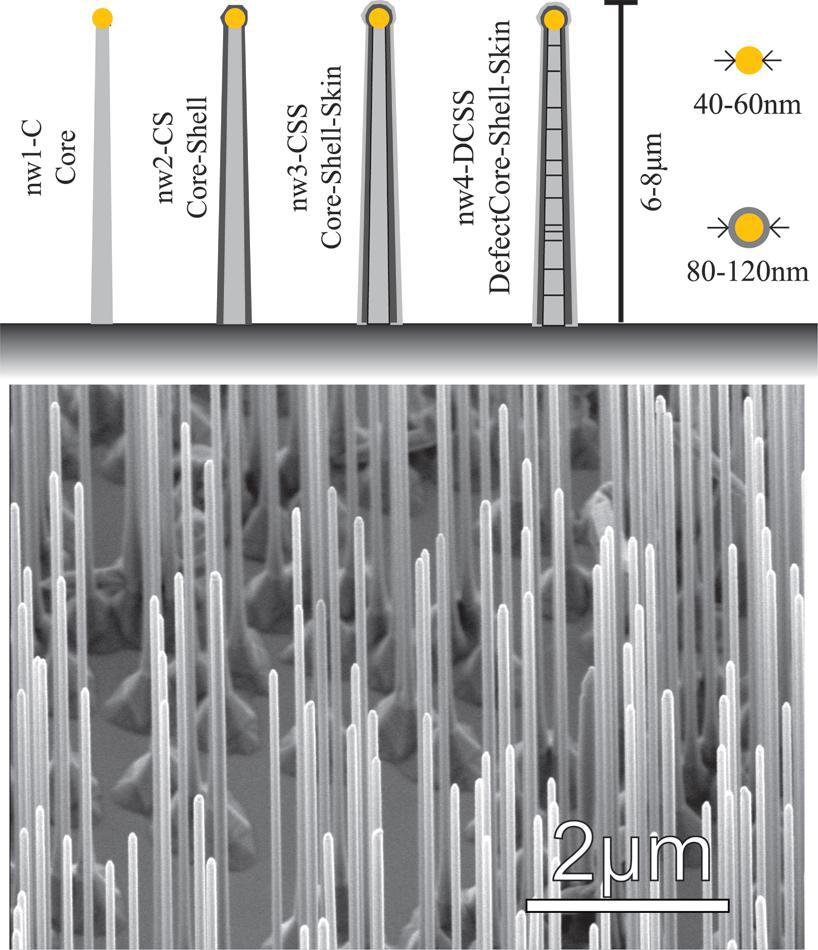
\includegraphics[width=0.6\linewidth]{NNWfromArticle}}
					\caption{СЭМ фотография образцов и их схематичное изображение. Рисунок взят из статьи \cite{CurrentLifetime}}
				\label{ris:NNWfromArticle}
				\end{figure}
				Первые три типа были выращены при двухтемпературном режиме: nw1-C - обычные ННК на основе $GaAs$, nw2-CS - ННК на основе $GaAs$ с шубой $AlGaAs$ толщиной $\sim$ 30 нм, а на образце nw3-CSS поверх шубы $AlGaAs$ был еще нанесен тонкий слой $GaAs$ примерно 5 нм. Четвертый образец nw4-DCSS по структуре такой же как nw3-CSS, но выращен при однотемпературном режиме и поэтому подвержен двойниковому дефекту плотности.\par
				Эксперимент показал, что покрытие шубой $AlGaAs$ ядра ННК на основе $GaAs$ увеличивает время жизни фотопроводимости примерно в четыре раза, кроме того, было установлено, что двутемпературный режим роста ННК увеличивает время жизни фотопроводимости на значительную величину. Для того чтобы оценить это время авторы использовали простую одноэкспоненциальную модель $\Delta E(\tau)/E = A Exp(-\tau/\tau_c)$. Но такая модель не дала им возможность оценить вклад бездефектного роста и в то же время воздействие верхнего слоя ($AlGaAs$). Чтобы установить влияние типа роста ННК и его структуры была предложена следующая модель:
				\begin{equation}\label{ModelOfChanges}
					\begin{cases}
   					\frac{dN}{dt} = -\frac{N}{\tau_{intrincic}} - \frac{N}{\tau_{NW}} - \gamma NT \\
					\frac{dT}{dt} = - \gamma NT \\
					\text{Начальные условия: } N(0) = N_i, T(0) = T_i
 					\end{cases}
				\end{equation}
				Где $N$ - концентрация неравновесных носителей заряда, а $T$ плотность свободных уровней ловушек. Первый член в уравнении для изменения плотности в единицу времени - это член отвечающий за объемную рекомбинацию проходящую за время $\tau_{intrincic} = 3 \text{ нс}$. Второй член в этом уравнении учитывает вклад ненасыщенной рекомбинации, которая возникает только в ННК. Третий член описывает захват заряда и рекомбинацию на поверхностных ловушках с коэффициентом связи $\gamma$, так же третий член - это скорость, с которой убывает концентрация поверхностных незанятых состояний ловушек. Подобранные параметры для уравнения (\ref{ModelOfChanges}) согласующиеся с экспериментальными измерениями позволили определить вклад типа роста и поверхностного слоя с большей шириной запрещенной зоны, эти параметры приведены в таблице \ref{CoefficientsFromModelOfChanges}.
\begin{table}[h]
\centering
\caption{Таблица параметров из работы \cite{CurrentLifetime}}
\label{CoefficientsFromModelOfChanges}
\begin{tabular}{@{}cc@{}}
\toprule
Параметр                         & Значение                          \\ \midrule
$\gamma$                           & $1.62 *10^{-7}$ $\text{см}^3\text{с}^{-1}$ \\
$\tau_{NW[1T]}$             & 10.2 пс                           \\
$\tau_{NW[2T]}$             & 28.2 пс                           \\
$T_{i[CS]}/T_{i[C]}$				   & 0.182                             \\ \bottomrule
\end{tabular}
\end{table}
В этой таблице $\tau_{NW[1T]}$ это время про которое говорилось выше, но применительно к ННК выращенным однотемпературным методом, а $\tau_{NW[2T]}$ для двутемпературного. $T_{i[CS]}$ и $T_{i[C]}$ это изначальная концентрация ловушек для ННК покрытых шубой и образцов типа nw1-C.
По определенным параметрам (таблица \ref{CoefficientsFromModelOfChanges}) авторы \cite{CurrentLifetime} сделали вывод о том, что покрытие шубой $AlGaAs$ ядра ННК на основе $GaAs$ уменьшает концентрацию свободных уровней поверхностных ловушек, а так же о том, что время жизни фотопроводимости увеличивается при уменьшении двойниковых дефектов в ядре ННК.\par
				Кроме времени жизни фотопроводимости в этой работе так же была оценена подвижность свободных носителей заряда во всех четырех типах ННК. Для этого экспериментально были измерены спектры фотопроводимости в ТГц области для каждого из четырех типов образцов. После чего экспериментальные данные были аппроксимированы уравнением для фотоиндуцированной проводимости, учитывающем вклад отклика свободных друдевских носителей и поверхностных плазмонов $\Delta\sigma = (\sigma_{Drude} + \sigma_{Plasmon})$.
				\begin{equation}\label{ModelOfConductivity}
					\begin{cases}
					\sigma_{Drude} = \frac{i N_d e^2 \omega}{m(\omega^2 + i \omega \Gamma)} \\
					\sigma_{Plasmon} = \frac{i N_p e^2 \omega}{m(\omega^2 - \omega_0^2 + i \omega \Gamma)}
 					\end{cases}
				\end{equation}
				Здесь $N_d$ и $N_p$ представляют концентрацию свободных носителей в друдевской моде и в плазмонной соответственно, a $\omega_0$ это плазмонная частота и $\Gamma$ - это обратное время релаксации электрона по импульсу. Определив с помощью аппроксимации экспериментальных данных моделью (\ref{ModelOfConductivity}) коэффициента $\gamma$, можно оценить подвижность $\mu = \frac{e}{m \Gamma}$. Для каждого типа образцов подвижность приведена в таблице \ref{MobilityFromArtycle}.
\begin{table}[h]
\centering
\caption{Таблица оценки подвижности на основе данных работы \cite{CurrentLifetime}}
\label{MobilityFromArtycle}
\begin{tabular}{@{}cc@{}}
\toprule
тип ННК		& Подвижность  $\text{см}^2/(\text{В} \text{с})$\\
\midrule
nw1-C                           & 1850\\
nw2-CS             				& 1650\\
nw3-CSS             			& 2250\\
nw4-DCSS				   		& 1200\\
\bottomrule
\end{tabular}
\end{table}
Из этих данных следует, что двухтемпературный рост вдвое увеличивает проводимость для ННК на основе $GaAs$ покрытых шубой $AlGaAs$ и тонким слоем $GaAs$. Кроме того, видно, что вообще говоря подвижность электронов различна в ННК покрытых шубой и обычных ННК. Первое объясняется тем, что при двутемпературном росте ННК значительно менее подвержены двойниковым дефектам. Второе, по предположению авторов \cite{CurrentLifetime} вызвано адсорбцией кислорода из ядра ННК $GaAs$ в шубу $AlGaAs$, при этом процессе адсорбция кислорода приводит к увеличению подвижности зарядов.\par
				Таким образом, авторы продемонстрировали один из способов изучения сверхбыстрой динамики носителей заряда в ННК на основе полупроводниковых материалов и получили интересные научно-практические результаты о способах изготовления ННК. Но в их работе нет никакой оценки того, как на подвижность носителей заряда в ННК могут влиять безызлучательные ионизованные центры.
			\subsection{Вклад безызлучательных ионизованных центров в электрическую проводимость в ННК.}
				В работе \cite{NonradiativeCenters} экспериментально продемонстрировано то, что в ННК на основе $GaAs$, выращенных методом газофазной эпитаксии, в транспорт носителей существенный вклад вносит механизм транспорта за счет ловушек. Авторы определили, что в отличии от тонких пленок на основе $GaAs$, в ННК на основе того же материала на транспорт оказывает существенно большее влияние дефекты в объеме. По их предположению это происходит в связи с тем, что поверхностные состояния в ННК на основе $GaAs$ полностью обедняют объем нанопровода, что позволяет ловушкам даже при небольшой плотности влиять на транспорт носителей.\par
				Чтобы получить больше информации о том, как именно влияют безызлучательные ионизованные центры на транспорт носителей в ННК и какой вклад носит процесс захвата носителей заряда на уровни этих центров, метода использованого в \cite{NonradiativeCenters} недостаточно. Для этих целей лучше подходит метод optical-pump terahertz generation-probe time-domain spectroscopy, который будет описан в основной части.
		\section{Генерация ТГц излучения}
			Метод, optical-pump terahertz generation-probe time-domain spectroscopy, который применяется в данной работе основан на генерации и детектировании ТГц излучения возбуждаемого фемтосекундным оптическим импульсом от образца, в котором помимо прочего возбуждается неравновесная электронная плазма. Поэтому в этой работе необходимо описать способы генерации импульсов ТГц излучения под действием фемтосекундных оптических импульсов.
			\subsection{Генерация импульсного ТГц излучения, как процесс оптического выпрямления}
				В средах с оптической нелинейностью второго порядка $\chi^{(2)}$ возможен процесс оптического выпрямления, когда под действием монохроматического оптического излучения, в среде возникает поляризация на нулевой частоте.
				\begin{equation}\label{Polarisation}
					P_i^{(2)}(0) = \chi^{(2)}_{i,j,k}(\omega - \omega)E_j(\omega)E_k(\omega)^*
				\end{equation}
				При распространении лазерного импульса, распространяющегося в среде с квадратичной нелинейностью будут возникать компоненты электрического поля, наведенного поляризацией вида (\ref{Polarisation})
				\begin{equation}\label{StraighteningElectricField}
					\Delta E_i(\vec{r},t) - 
					\frac{\varepsilon}{c^2}\frac{\partial^2 E_i(\vec{r},t)}{\partial t^2} = 
					- \frac{4 \pi}{c^2} \frac{\partial^2 P_i^{(2)}(\vec{r},t)}{\partial t^2}
				\end{equation}
				где $\varepsilon$ - диэлектрическая проницаемость среды, $P{(2)}$ - нелинейная поляризация,
наведенная лазерным импульсом. Преобразование Фурье от (\ref{StraighteningElectricField}) дает
				\begin{equation}\label{FourierStraighteningElectricField}
					\Delta \tilde{E}_i(\vec{r},\Omega) - 
					\frac{\varepsilon(\Omega)\Omega^2}{c^2}\frac{\partial^2 \tilde{E}_i(\vec{r},\Omega)}{\partial t^2} = 
					- \frac{4 \pi \Omega^2}{c^2} \frac{\partial^2 \tilde{P}_i^{(2)}(\vec{r},\Omega)}{\partial t^2}
				\end{equation}
				где $\Omega$ -разностная частота (частота генерируемой волны), $\tilde{E}_i(\vec{r},\Omega)$ - комплексная амплитуда компоненты электрического поля на разностной частоте, а $\tilde{P}_i^{(2)}(\vec{r},\Omega)$ комплексная амплитуда нелинейной поляризации вида (\ref{Polarisation})\par
				Из уравнения (\ref{FourierStraighteningElectricField}) видно, что излучение будет возникать на тех частотах, на которых соответствующая им комплексная амплитуда $\Omega^2 \tilde{P}_i^{(2)}(\vec{r},\Omega)$, отлична от нуля. Для фемтосекундного, гаусовского по времени лазерного импульса длительностью $2\tau$ можно получить, что $\Omega^2 \tilde{P}_i^{(2)}(\vec{r},\Omega) \sim \Omega^2 Exp\left( - \frac{\Omega^2}{(2/\tau)^2}\right)$ График этой функции представлен на Рис. \ref{ris:Fourier1}\par
				\begin{figure}[]
					\center{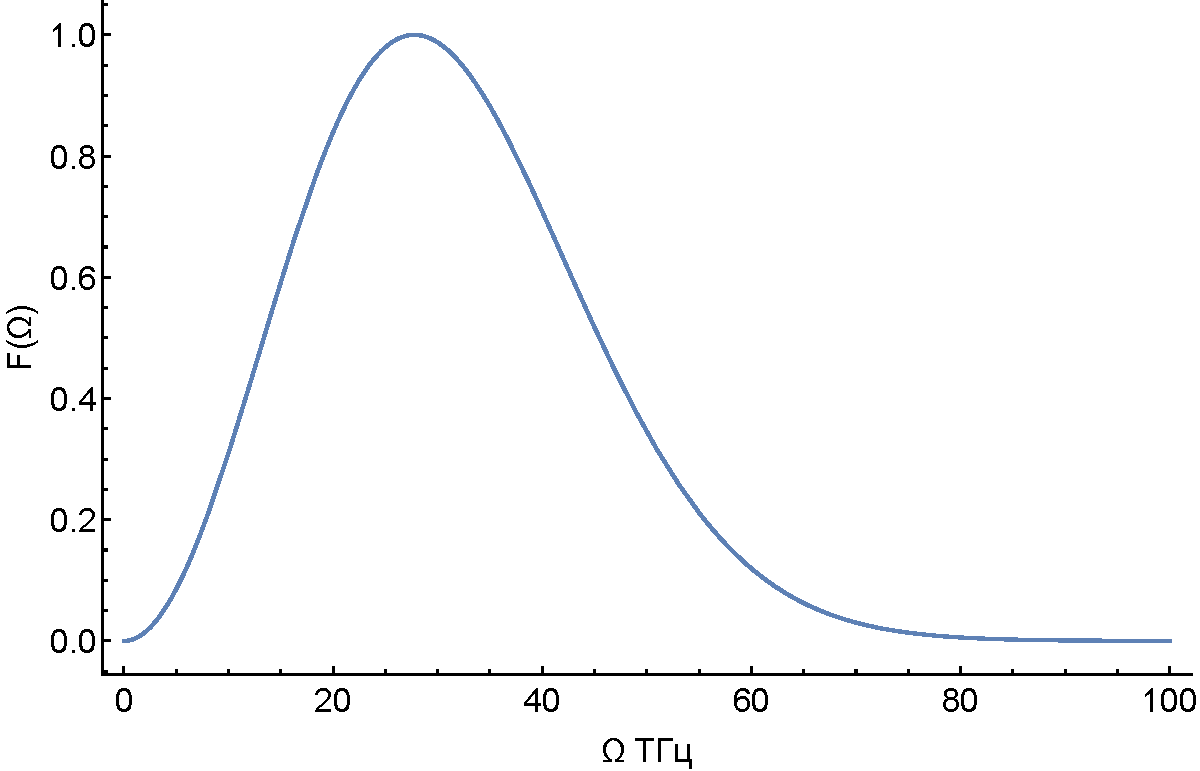
\includegraphics[width=0.65\linewidth]{Fourier1}}
					\caption{Амплитуда $\Omega^2 \tilde{P}_i^{(2)}(\vec{r},\Omega)$ для фемтосекундного лазерного импульса длительностью 120фc.}
				\label{ris:Fourier1}
				\end{figure}
				К примеру, для фемтосекундного лазерного импульса, длительностью 120 фс, максимум этой функции приходится на частоту $\sim$ 20 ТГц, а на частоте 1 ТГц значение функции составляет приблизительно 0.5\% от максимума.\par
				Таким образом, в нелинейно-оптических кристаллах с оптической нелинейностью второго порядка возможна генерация ТГц импульсов под действием фемтосекундного лазерного излучения.
			\subsection{Движение свободных носителей заряда в полупроводнике, индуцированное фемтосекундным лазерным импульсом, как источник ТГц излучения}
				Если энергия фотонов лазерного импульса больше ширины запрещенной зоны $E_g$ полупроводника, то при падении лазерного излучения на поверхность полупроводникового кристалла, происходит возбуждение электронов, сопровождающееся переходом электронов из валентной зоны в зону проводимости, в результате в поверхностном слое кристалла увеличивается концентрация свободных носителей, за счет возникающих под действием света электронно-дырочных пар. Однако помимо процесса генерации свободных носителей, происходит излучательная и безызлучательная рекомбинация электронно-дырочных пар, а также постоянная диффузия свободных носителей. Таким образом, при постоянной интенсивности падающего лазерного излучения устанавливается постоянная во времени концентрация свободных носителей вблизи облучаемой поверхности кристалла.\par
				Если длительность лазерного импульса много меньше времени релаксации населенности зоны проводимости, обусловленной рекомбинацией электронно-дырочных пар, то при падении импульсов на поверхность полупроводника, от импульса к импульсу происходят резкие всплески концентрации свободных носителей с дальнейшей релаксацией населенности зоны проводимости.\par
				В отсутствии внешнего электрического поля, возможны несколько механизмов генерации ТГц излучения, вызванной движением носителей заряда в полупроводнике.\par
				В некоторых полупроводниках около поверхности возникает направленное перпендикулярно поверхности электрическое поле. Поверхностное поле является результатом изменения границ зон электронных уровней вблизи поверхности. На Рис.  \ref{ris:GaAsSurfFields} изображена зонная структура кристалла $GaAs$ электронных энергетических уровней вблизи поверхности полупроводника.
				\begin{figure}[h]
					\center{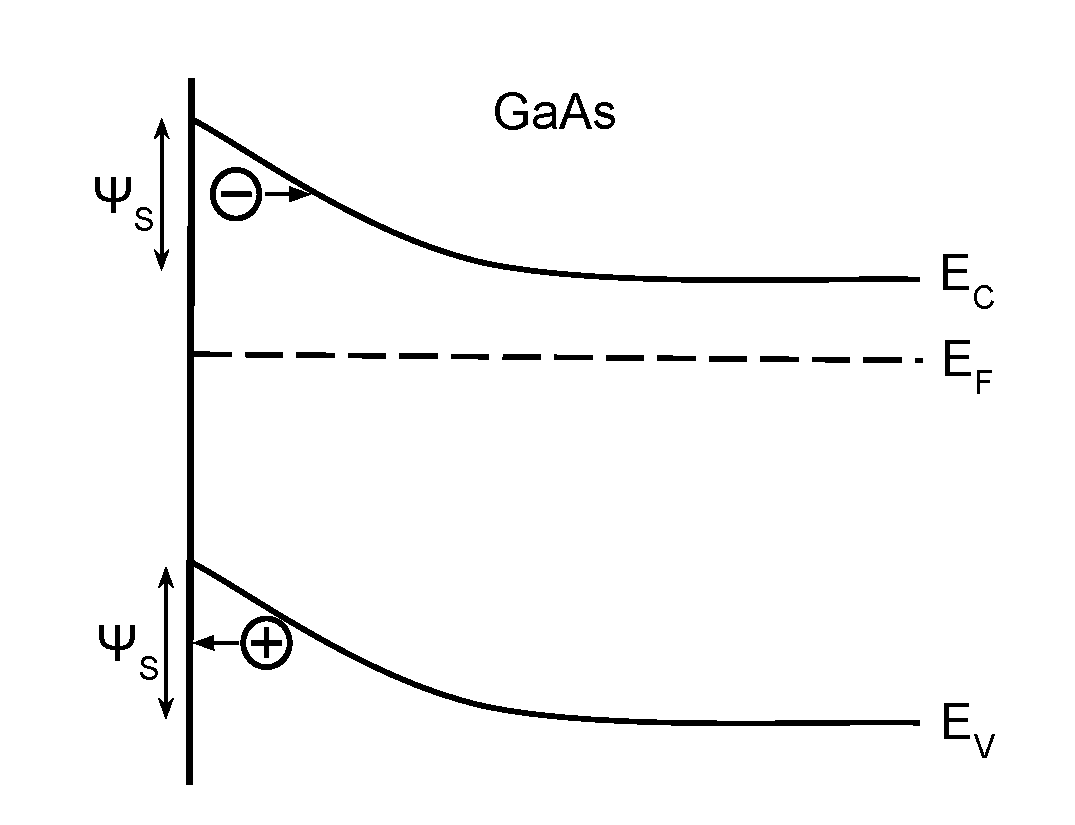
\includegraphics[width=0.65\linewidth]{GaAsSurfFields}}
					\caption{Зонная структура полупроводника $GaAs$ $n$ типа вблизи поверхности. $\Psi_S$ - поверхностный потенциал}
				\label{ris:GaAsSurfFields}
				\end{figure}
				При фотовозбуждении поверхностного слоя полупроводника, собственное электрическое поле, направленное перпендикулярно к поверхности, приводит в движение индуцированные светом свободные носители заряда. Таким образом, после начала импульса в поверхностном слое возникают сильнозатухающие колебания плазмы, которые и излучают электромагнитные волны в ТГц диапазоне. При использовании лазерных импульсов с длительностью порядка 100 фс, максимум спектральной плотности излучения соответствует примерно 1 ТГц.\par
				Амплитуда излученного терагерцового поля $E_{\text{ТГц}}(t)$ в направлении падающего оптического излучения $E_T$ и в направлении отраженного оптического луча $E_R$ в приближении модели диполя Герца в плосковолновом приближении
				\begin{equation}\label{THzAmplitude}
					E_R = \eta J \frac{Sin(\theta_1)}{Cos(\theta_1)+\frac{n_2}{n_1}Cos(\theta_2)}; \quad
					E_T = -\frac{n_1}{n_2}E_R T(\theta_2)
				\end{equation}
				где $\eta$ - импеданс образца, $\theta_1$ и $\theta_2$ углы отраженного и преломленного излучения, $n_1$ и $n_2$ показатели преломления воздуха и образца соответственно, а $J$ - фототок через обедненный слой, зависящий от угла падения оптического излучения, $T(\theta_2)$ - коэффициент пропускания границы раздела сред полупроводник-воздух. Выражение для фототока имеет следующий вид:
				\begin{equation}\label{CurrentDencity}
					J = \frac{\mu e}{h \nu} I_{ex}(1-R(\theta_{ex}))Cos(\theta_{ex})\int_0^{x}E_{in}(\xi)Exp(-\alpha \xi)dx
				\end{equation}
				где $\mu$ - подвижность носителей, $e$ – заряд электрона, $h \nu$ - энергия оптического
кванта, $I_{ex}$ - интенсивность оптического излучения, $\theta_{ex}$ - угол падения оптического излучения, $R(\theta_{ex})$ - коэффициент отражения оптического излучения от поверхности образца, $E_{in}$ - напряженность поверхностного электрического поля, $\alpha$ -коэффициент линейного поглощения оптического излучения.\par
				Второй, важный механизм генерации ТГц излучения от полупроводниковых материалов в результате движения свободных носителей заряда, индуцированного фемтосекундным лазерным импульсом - это генерация ТГц излучения в результате амбиполярной диффузии. Колебания плазмы под действием коротких световых импульсов в отсутствии
поверхностного поля возникают в результате разной скорости диффузии электронов и дырок в полупроводнике.\par
				В большинстве полупроводников электроны имеют больший коэффициент диффузии, чем дырки. Поэтому после	фотовозбуждения электроны диффундируют дальше вглубь полупроводника, создав тем самым диполь перпендикулярный поверхности полупроводника. Возникает электрическое поле (поле Дембера), вызывающее последующие сильнозатухающие колебания плазмы. При таком механизме генерации изменение типа легирования не влияет на знак генерируемого терагерцового поля $E_{\text{ТГц}}(t)$
			\subsection{Генерация ТГц излучения в ННК}
				В работе \cite{THzGeneration} исследованы механизмы генерации ТГц импульсов от массивов ННК при их фотовозбуждении фемтосекундными лазерными импульсами и установлено, что генерируемое ТГц излучение является результатом движения носителей в ННК, в частности установлено, что генерация ТГц излучения в ННК на основе $GaAs$ n типа и имеющих $Au$ слой на вершине, обусловлена сонаправленными дрейфовым и диффузионным токами, а генерация ТГц излучения в таких же ННК но p типа, связана с разнонаправленными дрейфовым и диффузионным токами. Исследуемые образцы представляли собой массивы ННК, которые были выращены на подложке $GaAs$ ориентации $(111)$ методом молекулярно пучковой эпитаксии с наночастицами золота в качестве катализатора.\par
				\begin{figure}[h]
					\center{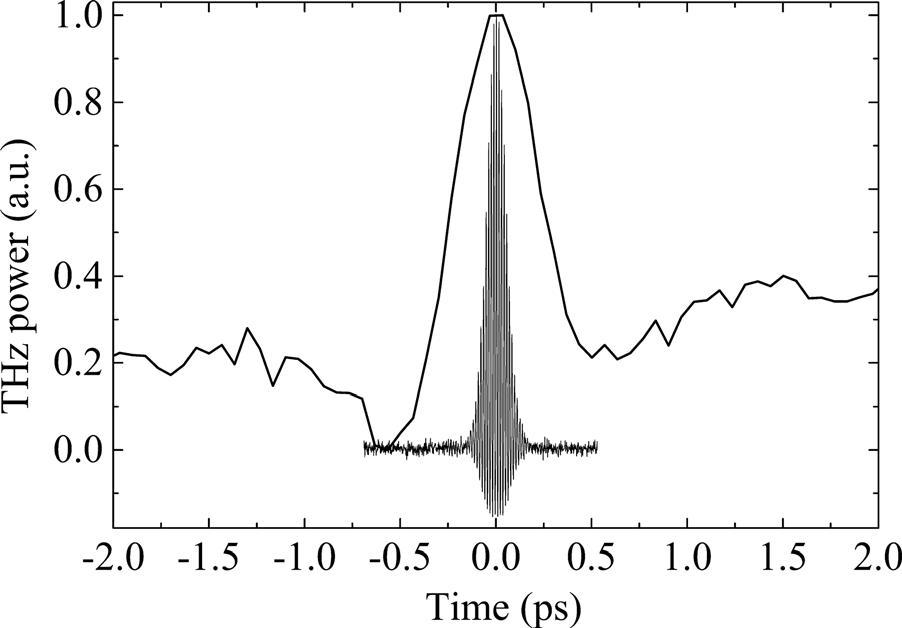
\includegraphics[width=0.65\linewidth]{THzPulseFromNNW}}
					\caption{Сравнение автокорреляционной функции ТГц импульса от ННК и фемтосекундного импульса, который использовался для фотовозбуждения образцов. График из статьи \cite{THzGeneration}.}
				\label{ris:THzPulseFromNNW}
				\end{figure}
				Для того, чтобы установить какие процессы в образцах отвечают за генерацию ТГц излучения, авторы измерили автокорреляционную функцию ТГц импульса. Оказалось, что при фотовозбуждении образцов фемтосекундными импульсами длительностью 90 фс при длине волны 800 нм, ширина автокорреляционного пика равна примерно 600 фс. На Рис. \ref{ris:THzPulseFromNNW} приведено сравнение фемтосекундного импульса и зарегистрированной автокорреляционной функции ТГц импульса. Из этого сравнения понятно, что генерация ТГц импульса от образцов ННК исследованных в работе происходит не за счет оптического выпрямления фемтосекундного импульса накачки. Так как при этом этом механизме генерации длительность ТГц импульса сопоставима с длительностью возбуждающего оптического импульса.\par
				\begin{figure}[h]
					\center{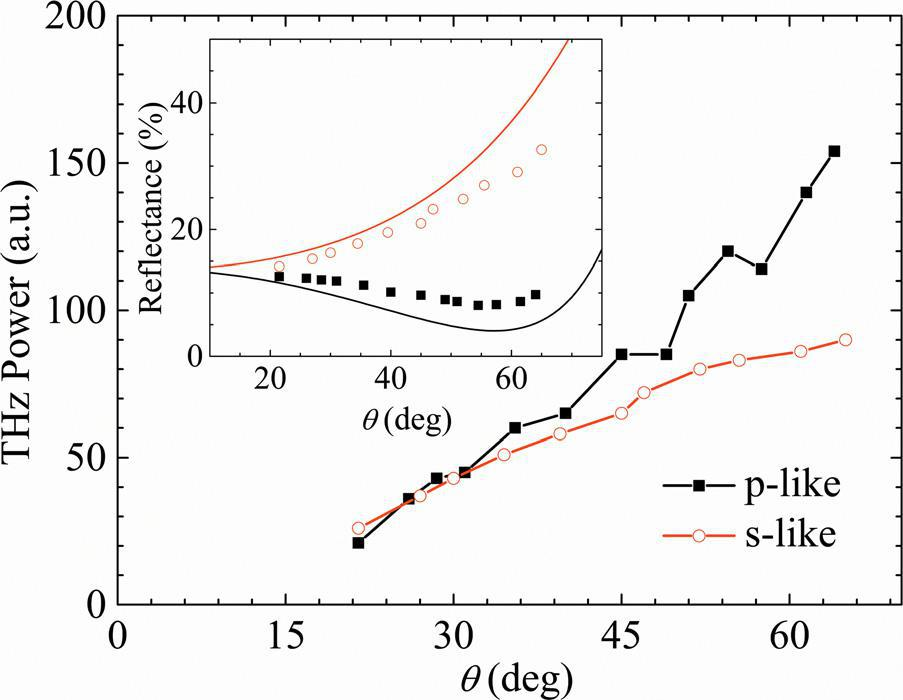
\includegraphics[width=0.65\linewidth]{ReflectiveNNW}}
					\caption{Угловая зависимость коэффициента отражения для s и p поляризации от ННК и от обьемного $GaAs$ на вставке. График из статьи \cite{THzGeneration}.}
				\label{ris:ReflectiveNNW}
				\end{figure}
				Таким образом установлено, что источником генерации ТГц импульсов от ННК, исследуемых в данной работе, является движение свободных носителей заряда в полупроводнике, индуцированное фемтосекундным оптическим импульсом. Чтобы выяснить, что источник ТГц импульсов - это движение носителей именно в ННК, а не в подложке, которая тоже на основе $GaAs$, авторы работы измерили угловую зависимость коэффициента отражения ТГц излучения для s и p поляризации. На графике Рис. \ref{ris:ReflectiveNNW} видно, что угловая зависимость коэффициента отражения от образцов не является Фринелевской, то есть отражение происходит не так, как от объемного $GaAs$. Это свидетельствует о том, что регистрируемое в экспериментах ТГц излучение результат дрейфового и диффузионного движения носителей именно в ННК, а не в $GaAs$ подложке.\par
				Так как именно движение свободных носителей и именно от ННК является источником ТГц излучения, при фозбуждении образцов, то зарегистрировав и проанализировав его можно понять, что происходит с носителями, как происходит их транспорт и их рекомбинация, а так же, каково время релаксации электрона по импульсу, а значит и подвижность электронов. Эта идея лежит в основе метода optical-pump terahertz generation-probe time-domain spectroscopy, но кроме оптического импульса используемого для генерации ТГц излучения используется еще один оптический импульс для генерации неравновесной плазмы носителей в ННК. Подробно этот метод описан в основной части.
	\chapter{Основная часть}
		\section{Описание метода и схема установки}\label{installation}
			Метод optical-pump terahertz generation-probe time-domain spectroscopy предполагает создание электронно-дырочной плазмы носителей в образце и детектирование изменения эффективности генерации ТГц импульса с момента генерации плазмы. Как было показано во введении, генерация ТГц излучения от ННК на основе $GaAs$ при фотовозбуждении их фемтосекундными импульсами происходит в следствии движения носителей заряда в ННК. А электронно-дырочная плазма влияет на эффективность генерации, причем это влияние может быть как положительным, так и отрицательным, это определяется многими факторами, такими как наличие глубоких уровней, величиной поверхностного потенциала и другими.\par
				\begin{figure}[h]
					\center{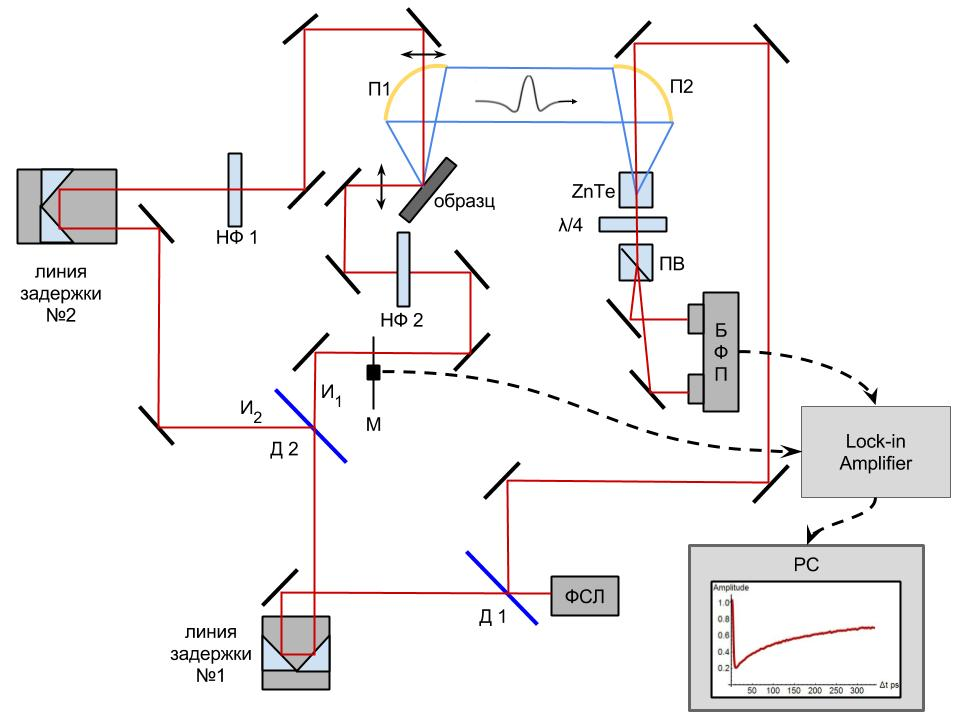
\includegraphics[width=0.65\linewidth]{Scheme}}
					\caption{Схема экспериментальной установки для реализации метода optical-pump terahertz generation-probe time-domain spectroscopy.}
				\label{ris:Scheme}
				\end{figure}
			Для того, чтобы реализовать экспериментальный метод была собрана установка, схема которой показана на Рис.  \ref{ris:Scheme}. Источником является фемтосекундный титан сапфировый лазер (ФСЛ) с центральной длиной волны светового импульса 795 нм, частотой следования 80 МГц и длительностью импульса 15 фс. Делитель (Д1) предназначен для того, чтобы отделить стробирующий импульс от импульса, который проходит первую линию задержки и делится (Д2) на два импульса, ($\text{И}_1$ и $\text{И}_2$). Первый $\text{И}_1$ моделируется (М) на частоте примерно 1 кГц, причем модулятор синхронизирован с синхронным усилителем, с помощью которого регистрируется сигнал с балансного фотоприемника (БФП). Второй импульс $\text{И}_2$ проходит через вторую линию задержки и через отверстие в параболоиде (П1) попадает на исследуемый образец. Таким образом оба импульса $\text{И}_1$ и $\text{И}_2$ попадают на образец, и как было описано ранее индуцируют движение носителей заряда в ННК, которое является источником ТГц излучения. Но из-за того, что только $\text{И}_1$ промодулирован на той частоте, на которой работает синхронный усилитель, сигнал регистрируемый балансным фотоприемником пропорционален амплитуде ТГц импульса генерируемого в результате фотовозбуждения ННК от $\text{И}_1$. При этом необходимо помнить, что когда промодулированный импульс попадает на образец, он модулирует среду с той частотой следования, с которой промодулирован сам. Это приводит к тому, что хотя импульс $\text{И}_2$ и не промодулирован на частоте синхронного усилителя, генерируемое им ТГц излучение синхронизируется за счет модуляции среды импульсом $\text{И}_1$ и поэтому синхронный усилитель его регистрирует. Вообще $\text{И}_2$ необходим только для генерации электронно-дырочной плазмы и его регистрация не желательна, для этой цели угол отражения $\text{И}_2$ совпадает с углом падения $\text{И}_1$, поэтому на параболоид П1 попадает ТГц излучение в основном то, которое является результатом возбуждения импульсом $\text{И}_1$.\par
			ТГц излучение от образца параболоидом П2 фокусируется на нелинейный кристалл $ZnTe$, через этот кристалл так же проходит излучение стробирующего импульса и за счет эффекта Керра и того, что стробирующий импульс поляризован (ну конечно он поляризован, это же лазерный импульс) его амплитуда меняется. После этого строб импульс проходит через пластинку $\lambda/4$ и разделяется призмой Волластона на два поляризованных перпендикулярно друг другу пучка и регистрируется балансным фотоприемником.\par
			С помощью программы написанной на LabVIEW, можно двигать обе подвижки, задавая шаг $\Delta x$, начальную позицию, количество усреднений и количество измерений. Первая подвижка изменяет оптический путь для $\text{И}_1$ и $\text{И}_2$, таким образом перемещая друг относительно друга импульсы генерации ТГц и стробирующий импульс, позволяя записывать волновую форму ТГц импульса. Вторая подвижка изменяет оптический путь только для $\text{И}_2$ и тем самым меняет момент генерации плазмы, относительно возбуждения образца импульсом $\text{И}_1$. В эксперименте использовались два метода, первый заключался в том, чтобы зафиксировать с помощью первой подвижки максимум ТГц импульса и после за счет второй подвижки менять момент генерации плазмы, таким образом измерялось, как эффективность генерации ТГц импульса меняется в результате генерации электронно-дырочной плазмы в ННК. Второй использованный метод заключался в том, чтобы с помощью второй подвижки зафиксировать момент генерации плазмы, а потом с помощью первой измерить волновую форму ТГц импульса. Второй подход использовался для того, чтобы снять спектры ТГц импульса и определить, вносит ли плазма изменения в механизм генерации ТГц излучения.\par
			С помощью нейтральных фильтров НФ1 и НФ2 можно менять мощность $\text{И}_1$ и $\text{И}_2$. В экспериментах интенсивность первого $\text{И}_1$ оптического импульса не превышала значений, при которых обеспечивался линейного отклик, т.е. в этой области уровня возбуждения имелась линейная зависимость максимальной амплитуды электрического поля ТГц импульса от средней мощности возбуждения. Таким образом, фактически изучалось влияние электронно-дырочной плазмы, генерируемой вторым  оптическим импульсом $\text{И}_2$ на эффективность генерации ТГц излучения.
		\section{Исследование ННК на основе $GaAs$}
			Исследование динамики эффективности генерации ТГц излучения от таких образцов интересно не только с фундаментальной точки зрения, но и с практической, так как упорядоченные массивы ННК на основе $GaAs$ являются эффективными эмиттерами ТГц излучения для сканирующей спектроскопии.
			\subsection{Описание образцов и метода их получения}
				ННК выращивались на подложках $GaAs$ р-типа с кристаллографической ориентацией $(111)$ методом газофазной эпитаксии из металл-органических соединений. Рост осуществлялся без предварительного нанесения слоя катализатора, но с помощью предварительной обработки подложек. Для этого, сначала на поверхность подложки осуществлялось осаждение слоя $SiO_x$ толщиной 40 нм методом плазмо-химического осаждения из газовой фазы на установке Oxford Instruments Plasmalab 80plus. Далее с помощью электронно-лучевой литографии сверхвысокого разрешения осуществлялось вскрытие окон в окисном слое диаметром 50 и 100 нм со скважностью 300, 600, 900, 1200, 1500, 1800 и 2100 нм. Вскрытые отверстия располагались в вершинах равностороннего треугольника. Рост ННК осуществлялся в атмосферном реакторе горизонтального типа на установке компании Thomas Swan. Соотношение потоков V/III было равно 200. Время роста варьировалось от 60 до 300 секунд. Температура роста была равна $480^\circ C$. На Рис. \ref{ris:OrderedSamples} представлены изображения периодических массивов ННК на основе $GaAs$, сделанных с помощью сканирующего электронного микроскопа. Видно, что ННК расположены в местах, где были вскрыты отверстия в $SiO_x$. ННК имеют вертикальные боковые стенки и обладают гексагональной морфологией. Как можно видеть на Рис. \ref{ris:OrderedSamples}, высота и диаметр нанокристаллов зависят от диаметра отверстия и их плотности. В итоге фактический диаметр ННК составил 80 и 160 нм. Размеры массива нанопроводов с заданной плотностью составляли 200х200 мкм.
				\begin{figure}[H]
					\center{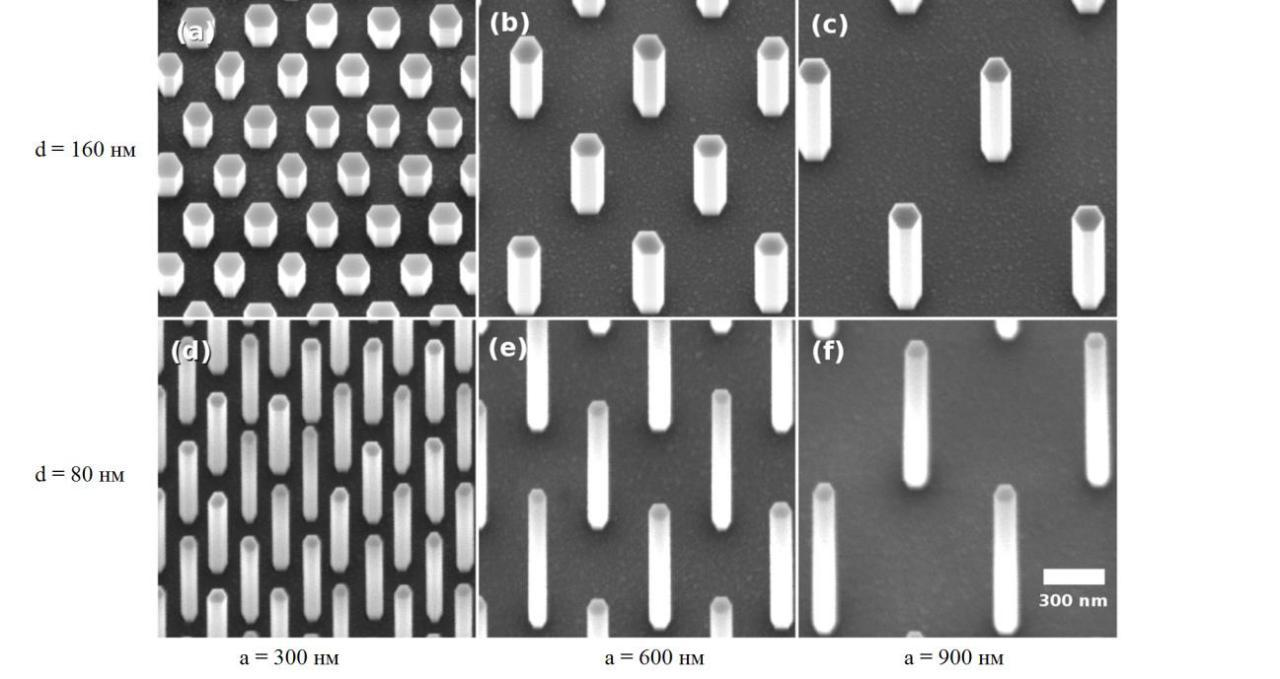
\includegraphics[width=0.85\linewidth]{OrderedSamples}}
					\caption{СЭМ изображения массивов ННК под углом $20^\circ$. Верхний ряд (a-c) – диаметр ННК составляет 160 нм, нижний ряд (d-f) – 80 нм. Расстояние между ННК: массивы a, d – 300 нм; b,e – 600 нм; c, f – 900 нм.}
				\label{ris:OrderedSamples}
				\end{figure}
%			\subsection{Зонная диаграмма ННК $GaAs$}
%				В ННК на основе $GaAs$ в объеме происходит обеднение электронами. Это приводит к тому, 
			\subsection{Зависимость эффективности генерации ТГц излучения от времени при возбуждении плазмы в образцах.}
				Для упорядоченных массивов ННК на основе $GaAs$, описание которых приведено выше, методом optical-pump terahertz generation-probe time-domain\\ spectroscopy, описанном в параграфе \ref{installation}, была измерена зависимость эффективности генерации ТГц импульса от времени генерации электронно дырочной плазмы. Была использована различная мощность накачки - что соответствует различной концентрации плазмы. На графиках Рис. \ref{ris:long600100}, Рис. \ref{ris:long120065} и Рис. \ref{ris:long1200100} отображены измеренные данные после нормировки, такой что эффективность генерации ТГц импульсов до возникновения плазмы в ННК принята за единицу.\par
				\begin{figure}[h]
					\center{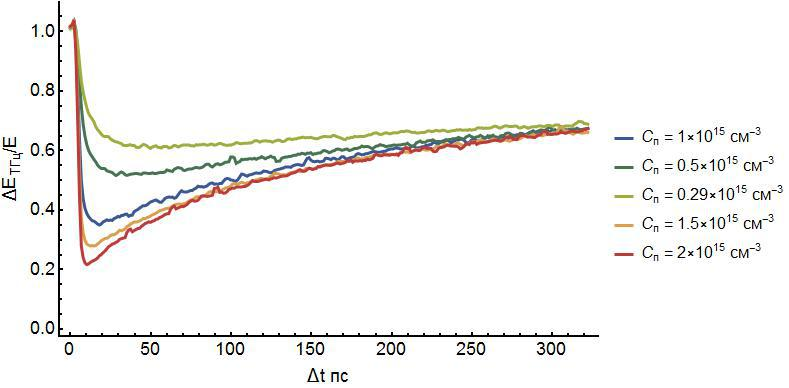
\includegraphics[width=0.85\linewidth]{long600100}}
					\caption{Изменение эффективности генерации ТГц излучения от времени возникновения плазмы в массиве ННК с параметрами $a = 600 \text{ нм, } d = 100 \text{ нм}$. В легенде к графику указанна концентрация плазмы.}
				\label{ris:long600100}
				\end{figure}
				\begin{figure}[h!]
					\center{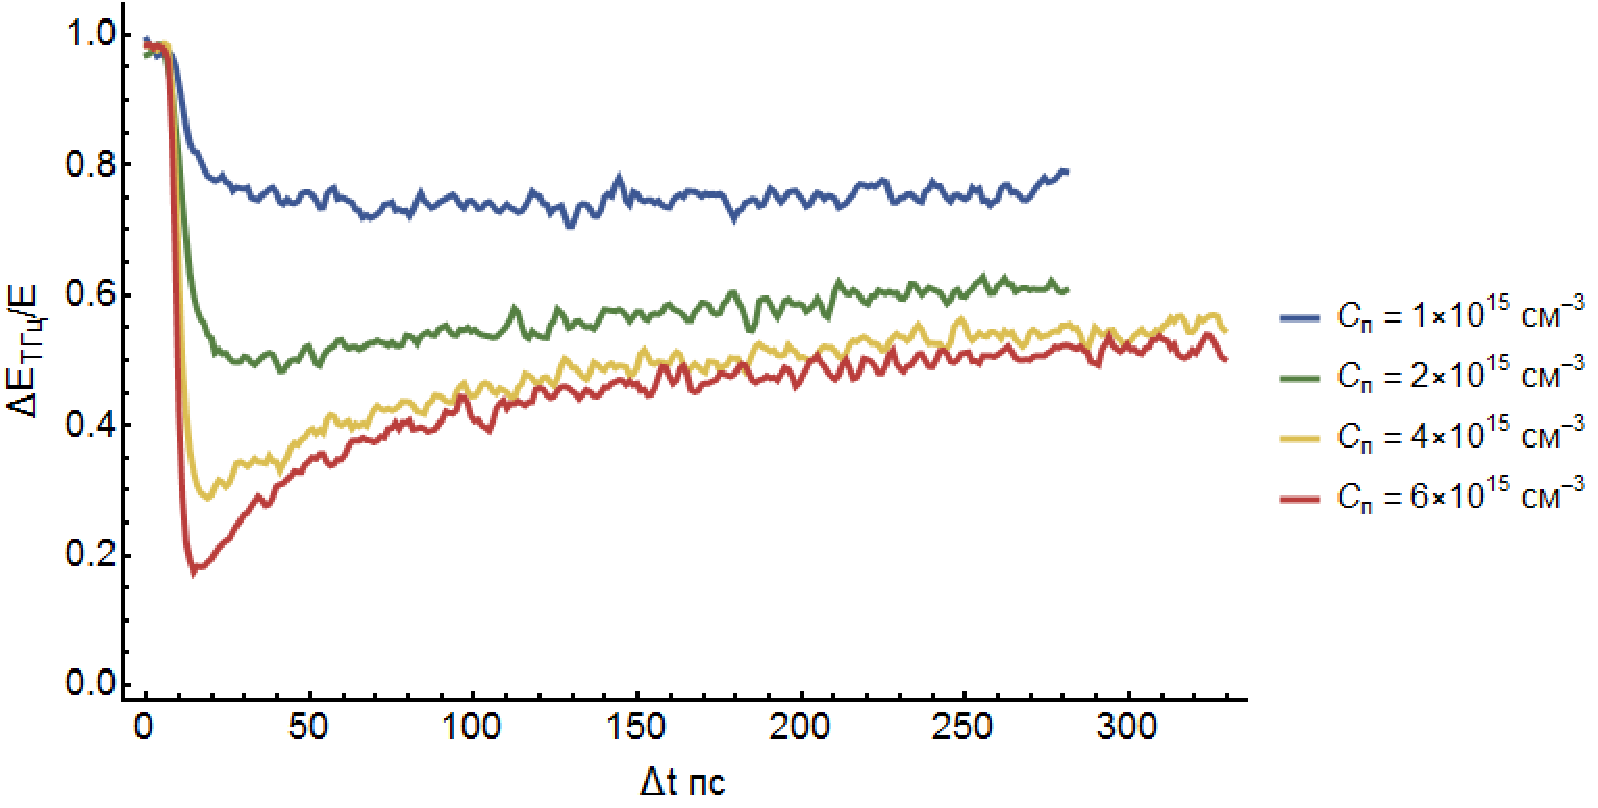
\includegraphics[width=0.85\linewidth]{long120065}}
					\caption{Изменение эффективности генерации ТГц излучения от времени возникновения плазмы в массиве ННК с параметрами $a = 1200 \text{ нм, } d = 65 \text{ нм}$. В легенде к графику указанна концентрация плазмы.}
				\label{ris:long120065}
				\end{figure}
				По графикам видно, что независимо от параметров массива: диаметра ННК и расстояния между ними, имеются два характерных участка, которые необходимо рассматривать отдельно. Первый - это резкий спад эффективности генерации ТГц, сразу после возникновения плазмы в ННК. Второй - это постепенное, неравномерное восстановление, которое к тому же зависит от концентрации возбуждаемой в образце плазмы. Последнее особенно хорошо видно на графиках Рис. \ref{ris:long120065}, еще при концентрации возбуждаемой плазмы $C_{\text{П}} = 2*10^{15} \text{см}^{-3}$ происходит постепенное восстановление, а уже при $C_{\text{П}} = 4*10^{15} \text{см}^{-3}$, в начальный момент происходит быстрое восстановление эффективности генерации ТГц, а после такое же, как и при концентрации плазмы в два раза меньшей.\par
				\begin{figure}[h!]
					\center{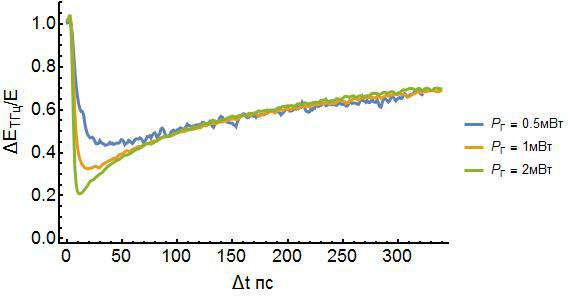
\includegraphics[width=0.85\linewidth]{long1200100}}
					\caption{Изменение эффективности генерации ТГц излучения от времени возникновения плазмы в массиве ННК с параметрами $a = 1200 \text{ нм, } d = 100 \text{ нм}$. В легенде к графику указанна концентрация плазмы.}
				\label{ris:long1200100}
				\end{figure}
				Кроме того, как будет описано дальше, на коротких временах есть еще один характерный участок, который связан с регистрацией ТГц импульсов, возбуждаемых при генерации электронно-дырочной плазмы. Это происходит в связи с модуляцией среды о которой уже говорилось в главе \ref{installation}. \par
				Таким образом, рассматривая зависимость эффективности генерации ТГц импульсов от времени генерации плазмы в ННК, необходимо выделять два временных промежутка, когда происходит резкий спад и когда происходит восстановление, характер которого зависит от концентрации плазмы. В следующих частях пойдет речь о каждом из этих участков по отдельности.
			\subsection{Спад эффективности - экранировка встроенного поля}
				Быстрый спад происходит на коротких временах порядка нескольких пикосекунд, тем не менее, с помощью экспериментального метода описанного в \ref{installation}, его можно зарегистрировать. Процесс уменьшения эффективности генерации регистрируется с разрешением примерно $50 \text{ фс}$, это не предельное временное разрешение, но уже достаточное, для регистрации этого процесса. Графики зависимости эффективности генерации ТГц излучения от ННК представлены на Рис. \ref{ris:short600100}, Рис. \ref{ris:short120065} и Рис. \ref{ris:short1200100}, данные нормированы так, что эффективность генерации ТГц импульсов до возникновения плазмы в ННК принята за единицу.\par
				\begin{figure}[h!]
					\center{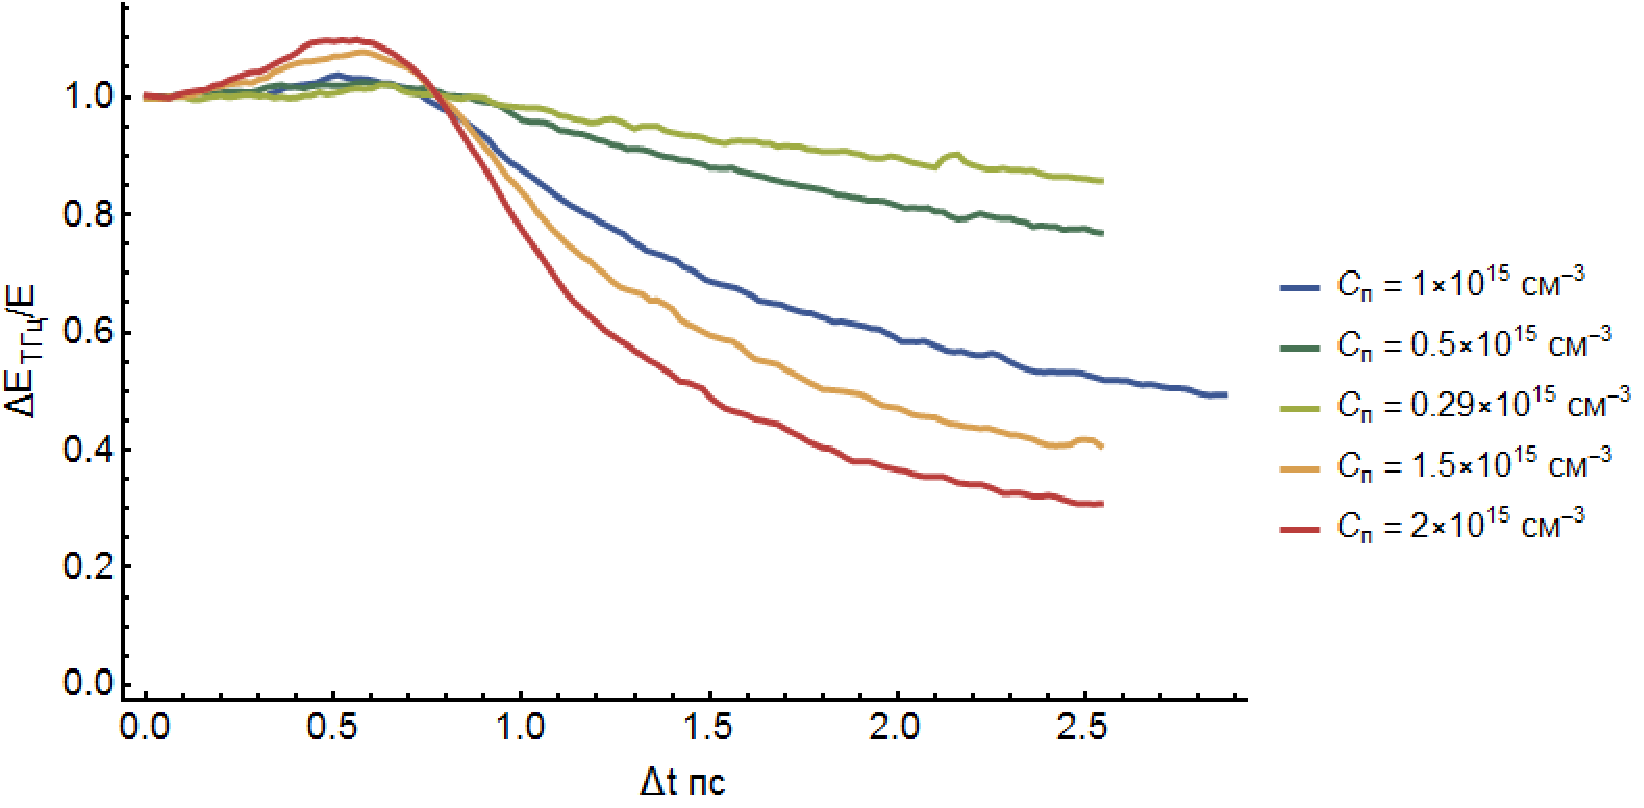
\includegraphics[width=0.85\linewidth]{short600100}}
					\caption{Спад эффективности генерации ТГц излучения после возникновения плазмы в массиве ННК с параметрами $a = 600 \text{ нм, } d = 100 \text{ нм}$.}
				\label{ris:short600100}
				\end{figure}
				\begin{figure}[h!]
					\center{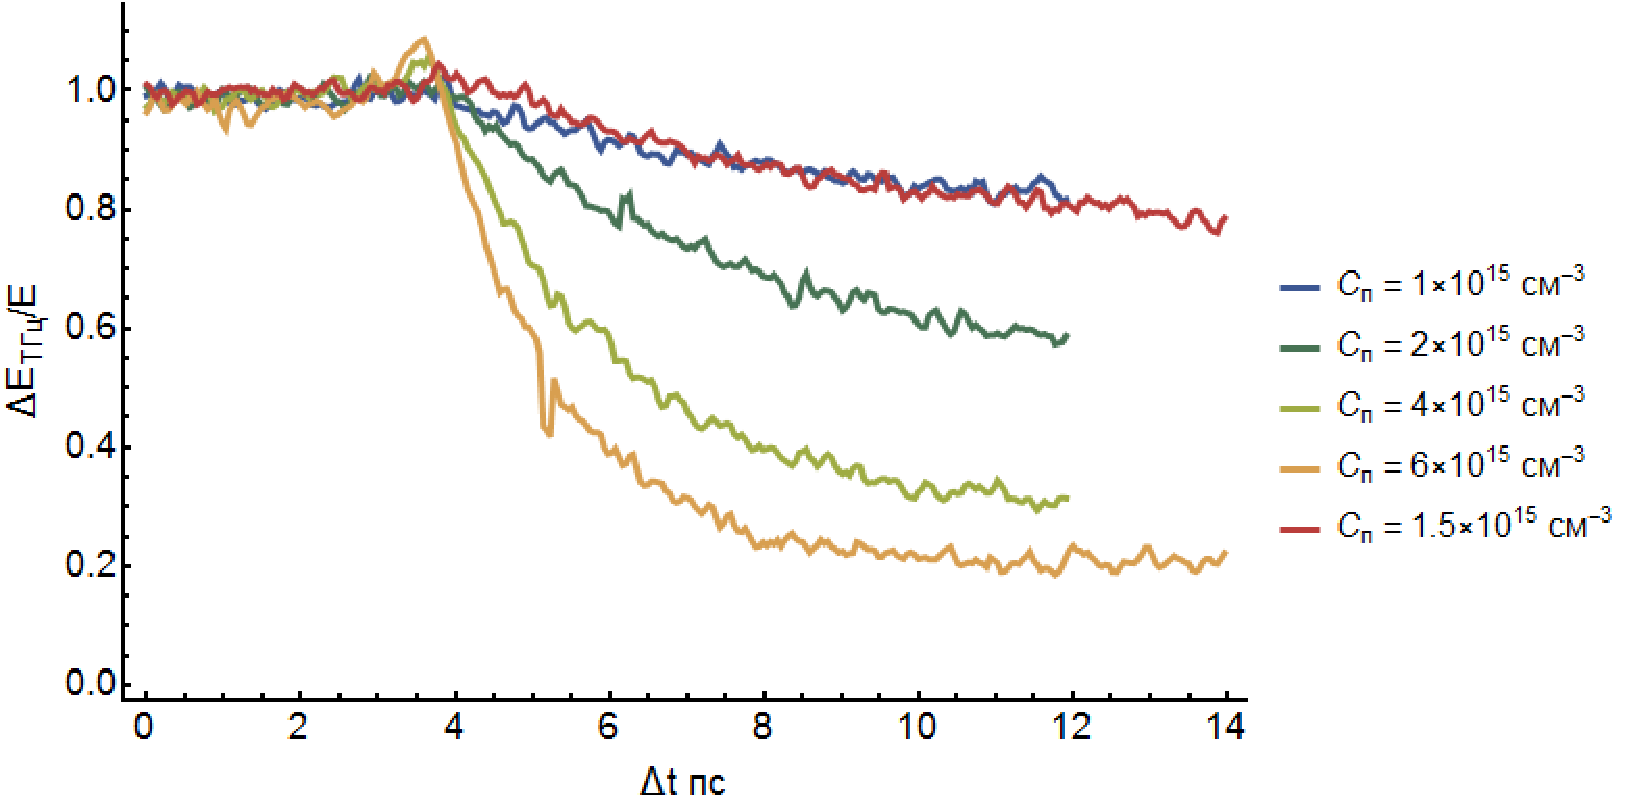
\includegraphics[width=0.85\linewidth]{short120065}}
					\caption{Спад эффективности генерации ТГц излучения после возникновения плазмы в массиве ННК с параметрами $a = 1200 \text{ нм, } d = 65 \text{ нм}$.}
				\label{ris:short120065}
				\end{figure}
				\begin{figure}[H]
					\center{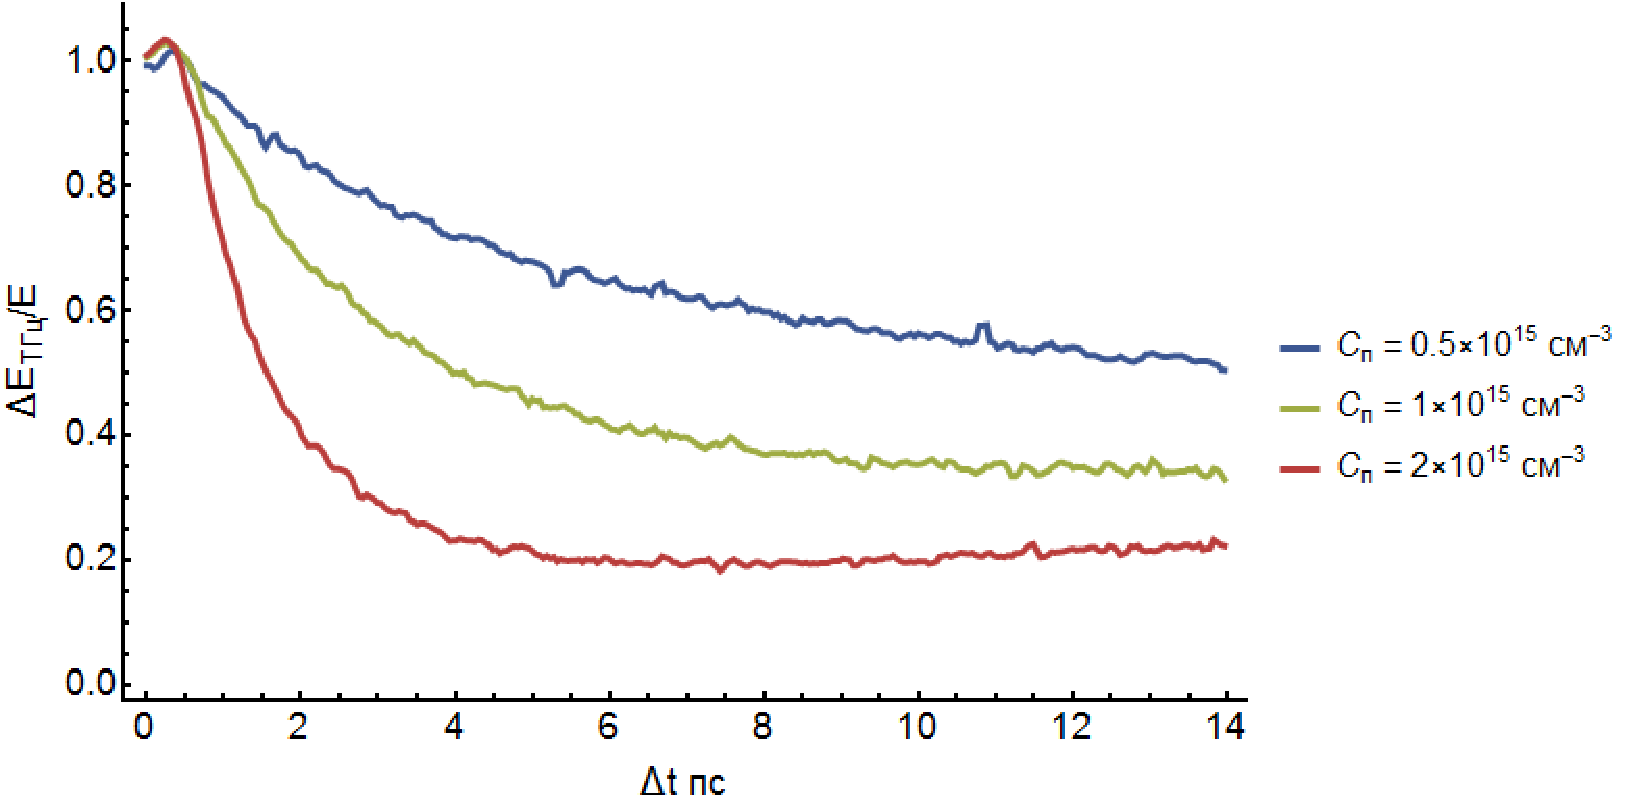
\includegraphics[width=0.85\linewidth]{short1200100}}
					\caption{Спад эффективности генерации ТГц излучения после возникновения плазмы в массиве ННК с параметрами $a = 1200 \text{ нм, } d = 100 \text{ нм}$.}
				\label{ris:short1200100}
				\end{figure}
				Амплитуда ТГц электромагнитной волны генерируемой от ННК, при возбуждении оптическими фемтосекундными импульсами, линейно зависит от напряженности встроенного электрического поля ННК, в случае равномерной или квазиравномерной напряженности встроенного электрического поля. В этом можно убедиться, используя соответствующее приближение и выражение \ref{CurrentDencity}, после чего, подставив полученный результат в \ref{THzAmplitude}, для $E_R$ получится \ref{ShortResult}
				\begin{equation}\label{ShortResult}
					E_R = \eta \frac{\mu e}{h \nu}\Phi(\theta_{ex}) E_{in} \left( \frac{1-e^{-a x}}{a} \right) \frac{Sin(\theta_1)}{Cos(\theta_1)+\frac{n_2}{n_1}Cos(\theta_2)}
				\end{equation}
				Где $\Phi(\theta_{ex}) = I_{ex}(1-R(\theta_{ex}))Cos(\theta_{ex})$, а $E_{in}$ - напряженность встроенного поверхностное поле в ННК. Поэтому, при регистрации изменение ТГц излучение он ННК, при возбуждении их фемтосекундными оптическими импульсами, регистрируется и изменение встроенного поля. Это изменение можно вычислить используя представление о наличии емкости поверхностного обедненного слоя.\par
				При перезарядке емкости, изменение напряженности локального электрического поля выражается следующим образом 
				\begin{equation}\label{Effectivity}
					\frac{\Delta E}{E} = Exp\left(-\left(\frac{e^2N\tau_S}{m^*\epsilon \epsilon_0 \eta}\right)t\right)
				\end{equation}
				Где $e$ -заряд электрона, $m^*$ – эффективная масса электрона, $N$ – концентрация неравновесных носителей заряда, $\epsilon$ – диэлектрическая проницаемость $GaAs$, $\eta$ - поправка к ёмкости с учетом краевых эффектов, $\tau_S$ время релаксации электрона по импульсу.\par
				Таким образом, по углу наклона графика зависимости эффективности генерации ТГц излучения от времени, с момента генерации плазмы, в логарифмическом масштабе ($Log\left(\frac{\Delta E}{E}\right)$ от $t$), можно оценить время релаксации электрона по импульсу ($\tau_S$) и обратную от этого величину - подвижность электронов в ННК $\mu_S$. На Рис. \ref{ris:shortLog600100}, Рис. \ref{ris:shortLog120065} и Рис. \ref{ris:short1200100} изображены графики зависимости $Log\left(\frac{\Delta E}{E}\right)$ от $t$, для массивов ННК с разными расстояниями между отдельными ННК и разным их диаметром.\par
				\begin{figure}[h]
					\center{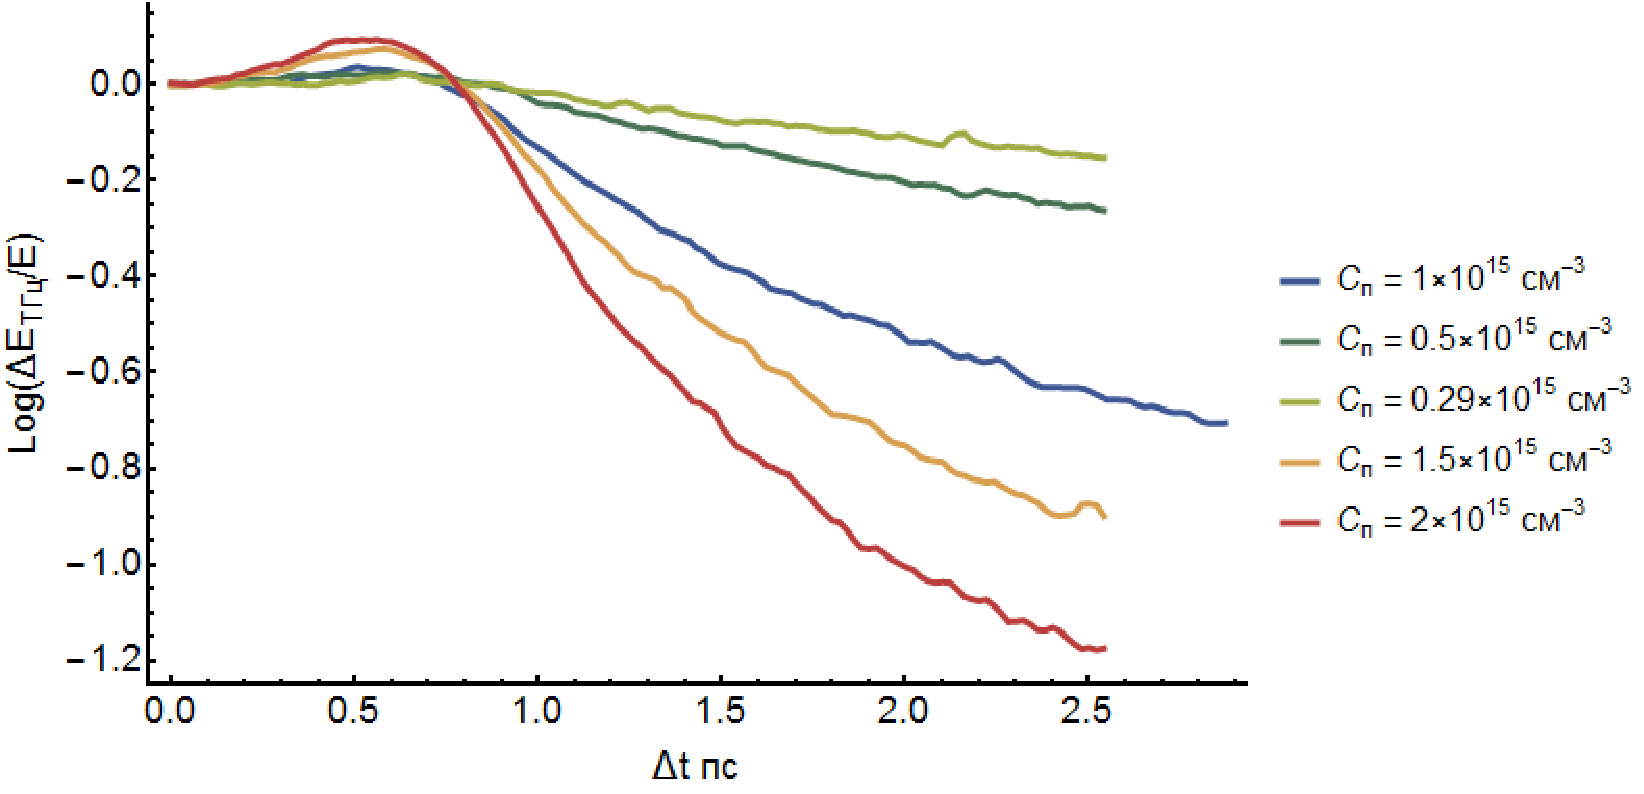
\includegraphics[width=0.85\linewidth]{shortLog600100}}
					\caption{Спад эффективности генерации ТГц излучения после возникновения плазмы в массиве ННК с параметрами $a = 600 \text{ нм, } d = 100 \text{ нм}$ в логарифмическом масштабе.}
				\label{ris:shortLog600100}
				\end{figure}
				\begin{figure}[h]
					\center{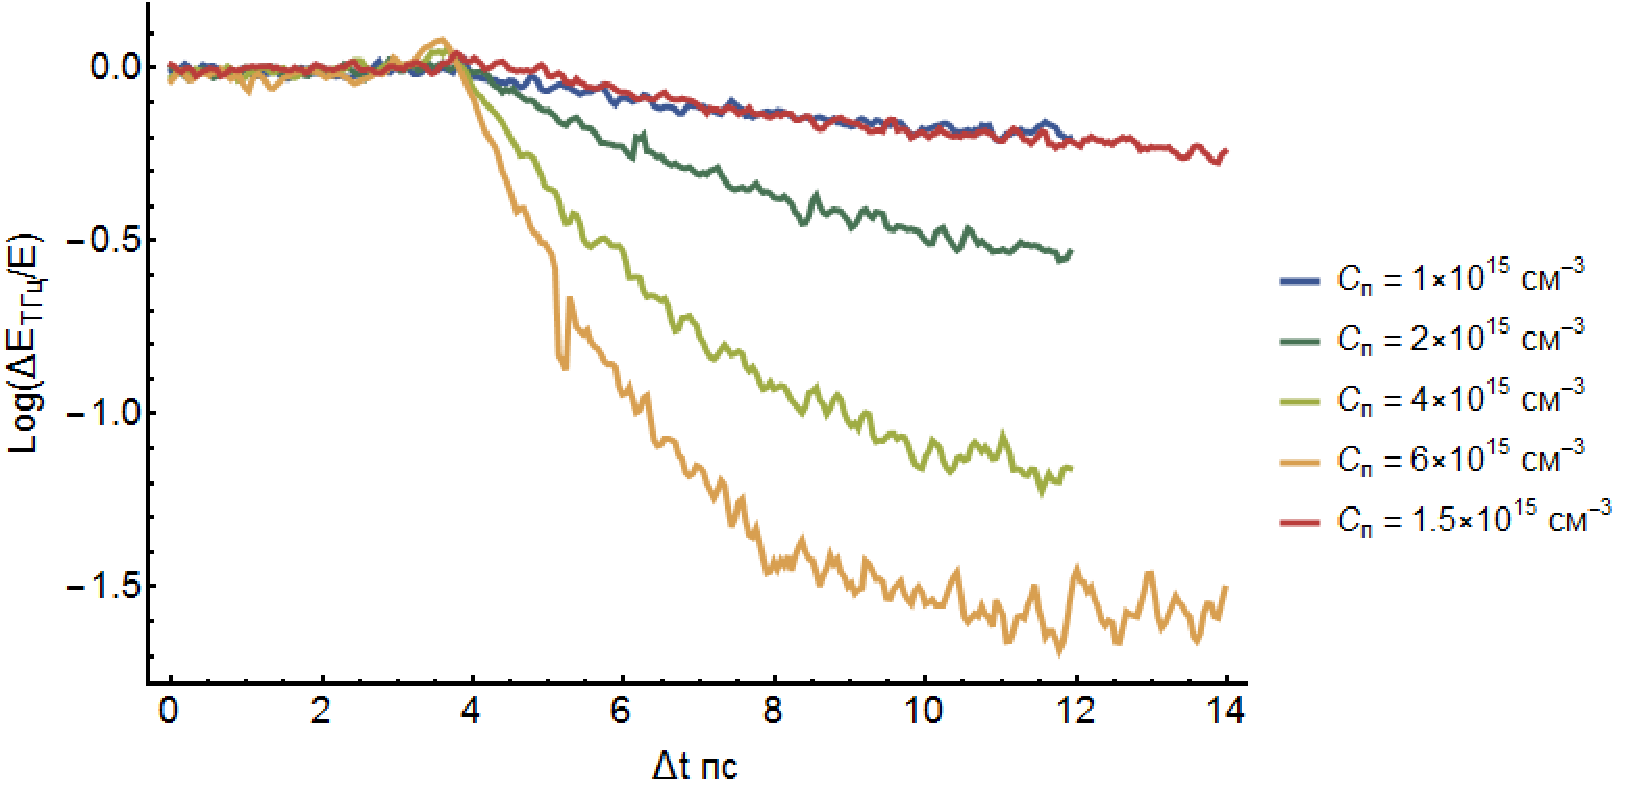
\includegraphics[width=0.85\linewidth]{shortLog120065}}
					\caption{Спад эффективности генерации ТГц излучения после возникновения плазмы в массиве ННК с параметрами $a = 1200 \text{ нм, } d = 65 \text{ нм}$ в логарифмическом масштабе.}
				\label{ris:shortLog120065}
				\end{figure}
				\begin{figure}[h!]
					\center{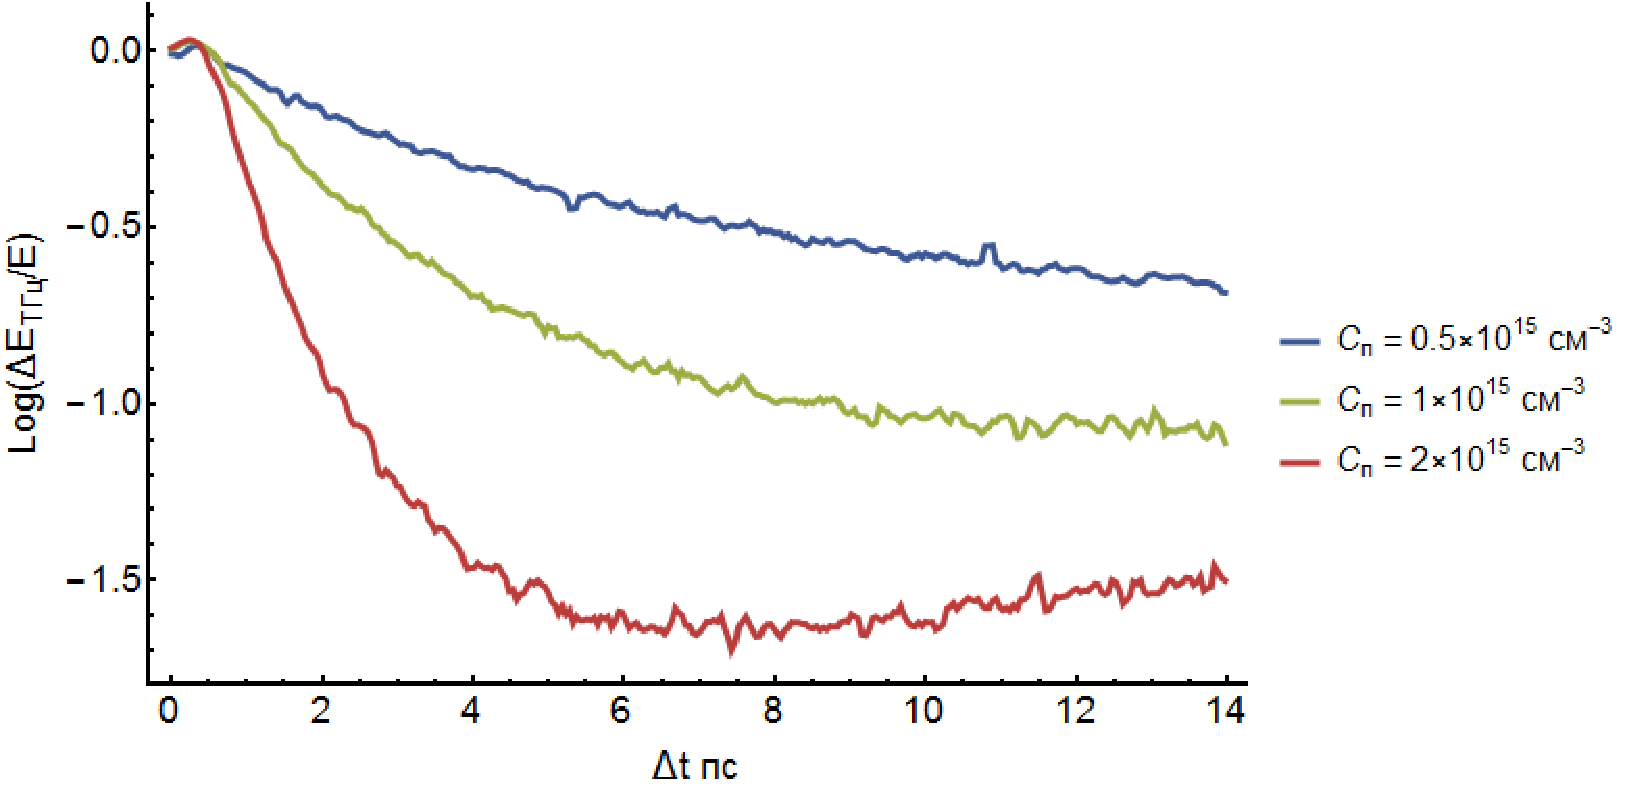
\includegraphics[width=0.85\linewidth]{shortLog1200100}}
					\caption{Спад эффективности генерации ТГц излучения после возникновения плазмы в массиве ННК с параметрами $a = 1200 \text{ нм, } d = 100 \text{ нм}$ в логарифмическом масштабе.}
				\label{ris:shortLog1200100}
				\end{figure}
				Для определения коэффициента наклона, по выделенным линейным участкам на рисунках \ref{ris:shortLog600100},  \ref{ris:shortLog120065} и \ref{ris:short1200100} и их линейной аппроксимации методом наименьших квадратов, можно построить зависимость тангенса угла наклона графиков, от концентрации неравновесной электронно-дырочной плазмы, для каждого из массивов ННК, рассмотренных выше. Эта зависимость линейна, так как для коэффициента наклона $\alpha$ можно записать $\alpha = \frac{e^2N\tau_S}{m^*\epsilon \epsilon_0 \eta}$. Результаты описанной выше процедуры приведены на 
			\subsection{Восстановление эффективности}
		\section{Исследование неупорядоченных массивов ННК на основе $GaAs$}
			\subsection{Описание образцов и метода их получения}
				Метод газофазной эпитаксии, ссылка на
				статью и короткое описание\par
				Ориентация $GaAs$, получившиеся образцы,
				фото СЭМ
			\newpage
			\subsection{Зависимость эффективности генерации ТГц излучения от времени при возбуждении плазмы в образцах.}
				Типичный вид динамики\par
				Динамика, для упорядоченных образцов,
				при разной мощности накачки\par
				Характерные участки (короткая и длинная
				динамика)\par
			\subsection{Спад эффективности - экранировка встроенного поля}
			\subsection{Восстановление эффективности}
		\section{Сравнение и анализ динамики носителей в разных образцах}
			Объяснение разницы в динамике
			\newpage
	\chapter{Заключение}
		\section{Положения дипломной работы}
			Все что удалось узнать, но в виде выражений и емких утверждений.
			\newpage
	\likechapter{Список сокращений и условных обозначений}
		\newpage
	\likechapter{Список терминов}
		\newpage
	\begin{thebibliography}{9}
		\bibitem{semicondNNW2006} Agarwal R., Lieber C. M. Semiconductor nanowires: optics and optoelectronics //Applied Physics A. – 2006. – Т. 85. – №. 3. – С. 209.
		\bibitem{NNWtransistors} Tomioka K., Yoshimura M., Fukui T. A III-V nanowire channel on silicon for high-performance vertical transistors //Nature. – 2012. – Т. 488. – №. 7410. – С. 189-192.
		\bibitem{singleNNWlaser} Duan X. et al. Single-nanowire electrically driven lasers //Nature. – 2003. – Т. 421. – №. 6920. – С. 241-245.
		\bibitem{THzGeneration} Trukhin V. N. et al. Generation of terahertz radiation in ordered arrays of GaAs nanowires //Applied Physics Letters. – 2015. – Т. 106. – №. 25. – С. 252104.
		\bibitem{SiliconNWContactPhenomena} Аверкиев Н.С., Шик А.Я.  Контактные явления в квантовых нитях и пористом кремнии//Физика и техника полупроводников. - 1996. - №.2 - С. 199
		\bibitem{CurrentLifetime} Parkinson P. et al. Carrier lifetime and mobility enhancement in nearly defectfree coreshell nanowires measured using time-resolved terahertz spectroscopy //Nano letters. – 2009. – Т. 9. – №. 9. – С. 3349-3353.
		\bibitem{NonradiativeCenters} Katzenmeyer A. M. et al. Poole-Frenkel effect and phonon-assisted tunneling in GaAs nanowires //Nano letters. – 2010. – Т. 10. – №. 12. – С. 4935-4938.
	\end{thebibliography}		
	\newpage 
	\likechapter{Приложения}
\end{document}



















